\documentclass{article}


\usepackage{graphicx} % Required for inserting images
\usepackage{siunitx}
\usepackage{biblatex} %Imports biblatex package
\usepackage{booktabs} % Required for tables
\usepackage{longtable}
\usepackage{appendix}
\usepackage{float}
\usepackage{amsmath}
\usepackage{rotating} % Required for sideways table
\usepackage{authblk}
\author[1]{Christian Magelssen}
\author[2]{Robert Reid}
\author[4]{Live Steinnes Luteberget}
\author[4]{Petter Jølstad}
\author[3]{Matthias Gilgien}
\author[4]{Per Haugen}
\affil[1]{Department of Mathematics, University X}
\affil[2]{Department of Biology, University Y}
\affil[4]{Department of Physical Performance, Norwegian School of Sport Sciences, Oslo, Norway}

\addbibresource{references.bib}


\title{The kinematic changes following a training intervention on pumping in slalom}
\begin{document}
\maketitle

\begin{abstract}
Slalom racers rely on effective strategies to bring them down the course in the shortest amount of time possible. One proposed strategy that skiers can use to achieve this goal is to pump themselves to higher velocities by extending their center of mass closer to the turn's axis of rotation from a laterally tilted position during the turn. However, the effectiveness of this proposed strategy and its potential magnitude are much debated. In a previous study, we found that skilled skiers (n=66) greatly improved their race times after training to pump on flats in slalom. Here, we ran a follow-up study and explored the kinematic changes that may explain this improvement in a smaller sample (n=18) of this larger pool of skiers, where we recorded the positions of the skiers using a local positioning system in the upper section of the course. Using a Bayesian estimation approach, we found that the velocity and acceleration profiles of the skiers changed greatly, with a change pattern consistent with what we would expect from pumping. We found little evidence that the total path length changed, however. Pumping to increase velocity on flats thus appears to be an important strategy for increasing velocity on flats.
    
\end{abstract}


\section{Introduction}
Slalom racers rely on effective strategies to bring them down the course in the shortest amount of time possible\cite{lesnik_best_2007, sporri_course_2012, sporri_turn_2012,supej_impact_2015, supej_relations_2006}.  Since situations in alpine skiing vary widely, skiers need different strategies for different scenarios. Therefore, skiers must acquire an extensive repertoire of strategies and learn to select the best strategies for each situation \cite{supej_impact_2015}. Consequently, both coaches and skiers have long strived to identify the most effective strategies for each scenario \cite{lemaster_skiers_1999, lemaster_ultimate_2010, joubert_how_1967,joubert_ski_1978, howe_new_2001, lind_physics_2013, muller_analysis_1994}, which is crucial for ski instruction and skill development.

One course section that stands out as pivotal for performance is the flat section\cite{supej_new_2011, supej_relations_2006}, where notable time differentials often emerge among skiers \cite{supej_impact_2015}. A defining characteristic of flat sections is that the amount of potential energy available for skiers to accelerate is lower than that available in steeper sections with steeper elevation profiles \cite{supej_differential_2008}. Therefore, it is important for skiers to minimize energy dissipation to maintain the highest possible velocity. Conventional strategies that the skier can employ to achieve this goal include carving instead of skidding and regulating the weight distribution along the length of the skies (fore/aft balance) during a turn\cite{reid_turn_2009, reid_kinematic_2010,supej_impact_2015, supej_differential_2008}.

Another, yet more debated, strategy is whether skiers can pump themselves to higher velocities in slalom \cite{lind_physics_2013, luginbuhl_identification_2023, mote_accelerations_1983}. According to Lind and Sanders' model \cite{lind_physics_2013}, skiers can increase their kinetic rotational energy during a turn by shortening the radius of the axis around which they rotate. This can be achieved by skiers extending their legs to move their center of mass closer to the rotational axis from a laterally inclined position (Fig. \ref{fig: design}b). Mechanically, this extension motion reduces the moment of inertia and consequently increases the skier's rotational kinetic energy and speed, assuming conservation of angular momentum. In their model, the increase in rotational kinetic energy from this motion is proportional to the amount of work exerted against the centrifugal force (from the skiers' frame of reference); thus, a larger extension movement results in a greater increase in rotational kinetic energy. Extending toward the axis of rotation can therefore potentially increase speed on flat terrain.

Yet, researchers have previously thought that the contribution of pumping to increase velocity is minimal and that it is a negotiable mechanism to increase speed and improve race times in slalom \cite{supej_differential_2008, supej_doba_2001}. The critics are directed towards that Lind and Sander's model neglects friction and that it should only work at low speeds \cite{supej_differential_2008, supej_how_2010}. Despite this, several studies have reported quantitative evidence that elite alpine skiers gain additional kinetic energy at the exit of the turn to—an increase that cannot be accounted for solely by their available potential energy preceding that moment \cite{reid_kinematic_2010, supej_differential_2008, supej_how_2010, supej_impact_2015}. Thus, pumping appears to be a mechanism that skilled skiers already exploit to increase speed to some extent. 

In two recent experiments, we have also provided evidence that skilled skiers can greatly improve their race times when performing the pumping strategy   \cite{magelssen_is_2022, christian_magelssen_reinforcement_2024}. In \textcite{magelssen_is_2022}, the skiers' were challenged to ski a slalom course in shorter time than if they skied straight down the hill from start to finish. If skiers could use a shorter time to ski the slalom course than  skiing straight down (meaning a longer path length), they must have increased their kinetic energy beyond the amount of potential energy available at the top of the slope, probably through the use of pumping technique. In that study, we reported that  skiers significantly improved their slalom course times compared with their straight-down gliding times over the course of the training sessions. For three of the ski teams participating in the study, we monitored the skiers using a local positioning system collecting position - time data in a five gate long section in the middle of the course. Here we ask whether we could explain this improvement through changes in kinematics. Because race time in alpine ski racing is a function of speed and path length, there are two ways in which these kinematic changes can manifest: alteration in path length or  speed. Therefore, the aim of this study was to investigate which of these explanations is most likely given our data and to explore the characteristics of these kinematic changes. We would expect that pumping would exert greater impact on the velocity than on the path length.

%whether shortening of the path or increase in speed lead to the shorter race times observed in \textcite{magelssen_is_2022} and hence indirectly assess if pumping to increase speed might have contributed to to the improved times in the slalom course from pre- to post test. 

\begin{figure}
    \centering
    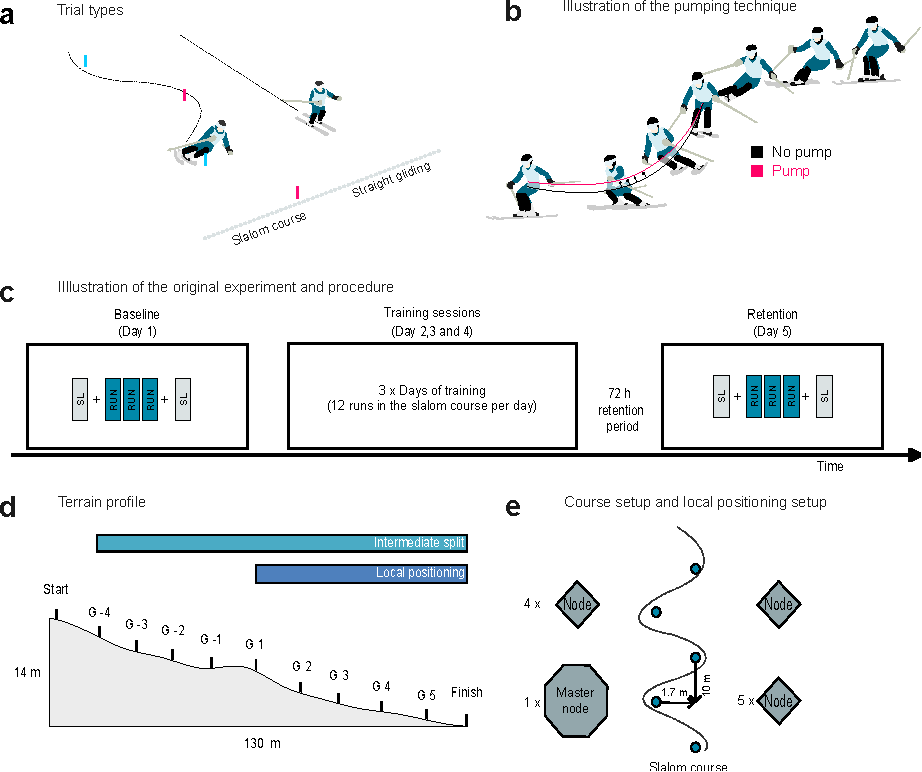
\includegraphics[width=1\linewidth]{figurer/figure_design_5.pdf}
    \caption{Illustration of the setup, experimental design and procedure. \textbf{a}. Illustration of the task and performance measures used in the study. The skiers' task was to ski faster in the slalom course than in straight gliding, which was also the measure used in our study. \textbf{b}. Illustration of the pumping technique. Skiers can achieve the pumping effect by extending their legs to move their center of mass closer to the rotation axis of the turn (from the black to the pink line). \textbf{c}. Illustration of the original experiment and procedure. The data analyzed in this study are from course B and are highlighted in blue. We analyzed only baseline and retention data but showed the training sessions to provide a complete illustration of the training intervention. See \cite{magelssen_is_2022} for a complete overview of the design and procedure \textbf{d}. Illustration of the course profile and the two analyzed sequences. \textbf{e}. Illustration of the setup of the local positioning system and the slalom course we have analyzed in this study.}
    \label{fig: design}
\end{figure}

\section{Methods}

\subsection*{Participants}
The participants in this study were eighteen alpine ski racers (mean age = 16.7 years, SD = 1.1; 7 females, 11 males) from three ski academies in Norway. These eighteen skiers formed a subset of a larger sample (66 skiers) from which we have already published results \cite{magelssen_is_2022}. We chose this subset of skiers because we only used the local positioning system at the upper section of the course for these skiers. With the exception of three skiers, all skiers had previously raced Fédération Internationale de Ski (FIS) races, with FIS points recorded (M = 115, SD = 31) in slalom. Their FIS points, however, may not accurately reflect their skill levels due to the challenges of organizing races during the COVID-19 pandemic, which limited opportunities to accumulate points.

\subsection{Setup}
The experiment took place on a 250-meter-long flat section of the race hill at the indoor ski hall in Oslo (\url{https://snooslo.no/}). Before each ski academy was tested, we watered this flat section to create a hard yet grippy snow surface, ensuring the most equal and consistent conditions throughout the intervention. Across the hill, we set up three slalom courses (courses A, B, and C) with the purpose of testing the contextual interference effect\cite{magelssen_is_2022}. See Appendix \ref{appendixa} for an overview and illustration of how we set the courses. Here, we report only data from Course B because it resembled a typical slalom course the most. This course featured a 1.7-meter gate offset and a 10-meter vertical distance (blue course in Fig. \ref{fig: design}e). 

We used a standardized starting procedure to minimize variation in entry speed. That is, the skiers started 20 meters before the first gate from a stationary position with the forebinding placed behind the start gate. Upon receiving clearance to start, skiers lifted their poles from the snow and skied straight down 10 meters from the hill until crossing the first photocell, which started the timer. Subsequently, skiers continued down the course. For the purposes of this study, a trial concluded when skiers crossed the second intermediate split (Fig. \ref{fig: design}d), although they continued skiing the rest of the course. The race time data were recorded using a wireless photocell timing system (HC Timing wiNode and wiTimer; Norway).

In addition to the timing system for recording times, we used a local positioning system to record the skiers' positions as they navigated the course section. To this end, we used Catapult ClearSky T6 (Catapult Sports; Australia). Initially, the local positioning system section covered the area just before the first photocell and until the second intermediate split (length: 90 m and width: 30 m). However, due to the narrowness of the ski hall in the upper part of the course, the wall was too close to the nodes, impeding signal reception until the skiers descended further down where the hall widened.  Consequently, we only have data from the local positioning system for a smaller section of the course. In Supplementary \ref{appendixd}, we elaborate on this challenge in more detail. For the setup of the local positioning system, we deployed ten nodes on each side of the hall (Fig. \ref{fig: design}d and e). One node served as the master node and was positioned on the skier's right side of the course. Since the Catapult ClearSky T6 only provides positional data in 2 dimensions (X and Y axes), we measured the elevation profile (Z) of the slope by taking point measurements every ten meters (at each gate) using a tachymeter (Leica Builder 509 Total Station, Leica Geosystems AG, Switzerland) and interpolating values between these points. We also used this tachymeter for the spatial calibration of the local positioning system. Each skier wore a manufactured-supplied vest that supported a lightweight (28 g) mobile node (firmware version: 1.40), measuring L: 40 mm × H: 52 mm × D: 14 mm.  The local positioning system provided positional data as skiers descended through the course section (sampling frequency \~10 Hz), enabling us to compute their velocity and path length. Compared to the Qualisys system, the local positioning system has been found to operate within the range of 0.21-0.35 m error in distance with an optimal setup (but much better with a suboptimal setup)\cite{luteberget_validity_2018}. This error might be too high for skiing, but to our defense, it was the only system we could use to record this amount of data at the time we undertook the study.

\subsection{Design and procedure}
The original study consisted of a five-day learning experiment with a three-day learning intervention on learning to pump in slalom (Fig. \ref{fig: design}c). On day 1, the skiers underwent a baseline test comprising a total of 9 runs (3 runs in the slalom course reported in this study), during which they received instructions to ski as quickly as possible down the course. During these runs, the skiers did not see their race times. Before and after the 9 runs in the slalom courses, the skiers performed a straight gliding run, where they descended the section straight down without any turns. Straight gliding was conducted in an upright, stationary posture to ensure a consistent drag area for each run (Fig.\ref{fig: design}a).

After the baseline test, all skiers gathered for a workshop where the principle of pumping was explained, and quantitative evidence of its effect was presented. Following this, the skiers underwent three days of training on this pumping strategy (12 trials per day, of which four were in the course reported in this study). During these sessions, the skiers received race times as feedback after each trial, expressed as the difference between course time and straight gliding run time. In the original learning experiment, we assigned the skiers to two learning groups. However, since no evidence for a treatment effect was found, we combined the groups in our analysis and henceforth only described the overall procedure.  Further specifics of the experiment and procedure can be found in the original study \cite{magelssen_is_2022}

After the three training sessions (days 2, 3, and 4), the skiers had a three-day break during which they did not ski (retention interval). Following this break, skiers underwent a retention test (same as baseline) consisting of a total of 9 runs (3 runs in the slalom course reported in this study). During this test, they received instructions to ski as quickly as possible down the courses, with no timing provided as feedback, similar to the baseline procedure. 


\subsection{Analysis}
The cleaning and processing of the data began with custom functions in MATLAB, which were developed, tested, and used in previous studies \cite{reid_kinematic_2010}. Subsequently, the files were imported into Python using the SciPy \cite{virtanen_scipy_2020} and pandas \cite{mckinney_pandas-powerful_2015} packages. During this import, some trials caused import problems in Python because they were not part of the experimental protocol (warm-up runs or freeski runs). In addition, in a few cases, the quality of the data from the local positioning signal was poor, preventing the calculations in MATLAB from proceeding. In both error cases, we manually removed the runs from the MATLAB file. After this processing step, the remaining data underwent two manual screening processes to verify the quality of the local positioning data. The first screening process involved removing all runs that did not match the experimental procedure, such as warm-up runs or runs where a skier did not finish (DNF) the run. In the second screening process, all runs were visually inspected to identify errors in the local positioning data. To aid in this detection, the race times in the section, the position coordinates, and the velocities of all the ski racers were plotted. All the runs we removed are documented, along with the reasons for their removal. An extensive report of this cleaning and validation process can be found at the Open Source Framework (OSF)  (\url{https://osf.io/egbpr}).

Our general statistical approach was to leverage multilevel modeling due to the hierarchical data structure of our data. This hierarchy was due to two sources: each skier had three runs in the slalom course on baseline and retention (by design), and the skiers were nested within three different ski academies that conducted the learning experiment together. We employed a Bayesian estimation approach because our goal was to describe the changes and interpret their effects rather than testing any hypothesis \cite{kruschke_bayesian_2018}, where we incorporated this multilevel information in our models. To determine the random effects structure, we used a design-driven approach where our choice of random effects was determined by the design of the experiment \cite{barr_learning_2021, barr_random_2013}. In some cases, this design-driven model formula failed to converge with the ski academy as a random effect  (that is, varying intercept, slope or smooth) due to few varying levels. Therefore, in these cases, we opted for a simpler model that excluded this multilevel information. To fit the models, we used the brms \cite{burkner_brms_2017} package in R \cite{r_core_team_r_2022}. We used weakly informative priors and performed prior predictive check simulations to inform our decisions. All models (including the priors) are reported in Supplementary \ref{appendixc} and the codes are available at OSF. To extract and visualize the draws from the model, we used the Tidybayes package \cite{kay_tidybayes_nodate}. We chose to report the average mean and contrast for a typical skier (that is, setting the random effects to zero when making posterior predictions). 

We used multilevel generalized additive models (GAMs) \cite{pedersen_hierarchical_2019, wood_generalized_2017} for most of our analyses. The reason for our choice is that GAMs allow greater flexibility in modeling nonlinear shapes in data and therefore better allow us to model our kinematic data. In general, a GAM model takes the form of $Y \sim \beta_0 + S(x)$, where $\beta_0$ represents an intercept term, and $S(x)$ is a smooth function of the predictor $x$. The smooth function $S(x)$ in the model is in turn composed of several simple basis functions ($K$), each with an estimated coefficient derived from the data. Researchers can model more complex shapes by adding many basis functions ($K$) to the data. With this approach, risk looms such that the model overfits the sample data and therefore leads to poor out-of-sample generalization. This risk is counteracted in the GAM by penalizing the coefficients of the basis functions such that the model effectively negotiates the tradeoff between the wiggly smoothers and generalizability. 

\subsubsection{Race times}
To analyze the race times, we conducted two statistical analyses. In the first model, we examined the time it took from the start to the second intermediate time, which was positioned just after the finish of the local positioning section (Intermediate section in Fig. \ref{fig: design}d). In this model, we predicted race time (measured as the time behind straight gliding in the respective session), with session (baseline, retention) as a fixed effect, and a random intercept and slope for skiers. Due to the limited number of levels in the ski group, we were unable to achieve model convergence with the ski group as a random intercept or slope, and therefore omitted this varying effect from the model. We coded session (baseline, retention) with an index coding approach to place equal uncertainty for both levels and to ease the process of setting sensible priors \cite{mcelreath_statistical_2018}.

For the second model, we analyzed the local positioning (Fig.\ref{fig: design}d) with the data from the local positioning system to determine whether the skiers also improved in this small section. These data were normalized to ensure an equal number of data points between the gates in the sequence. To model the race times in this section, we employed the difference between the time in the slalom course and the time straight down for the entire length of the section. We modeled this difference with a multilevel generalized additive model (GAM) as an average global smooth plus random smooth for each skier \cite{pedersen_hierarchical_2019}. We allowed the skiers to have their own random smooth because we know that kinematic data can vary significantly both between and within skiers \cite{federolf_quantifying_2012, supej_impact_2015, reid_kinematic_2010}.

\subsubsection{Velocity}
To calculate the resultant velocity of the three velocity vectors, we applied the Pythagorean theorem for each incremental change in $X$, $Y$, and $Z$ for the course section. Note that we constructed an artificial elevation profile (Z) of the slope by taking point measurements every ten meters (at each gate) using a tachymeter (Leica Builder 509 Total Station, Leica Geosystems AG, Switzerland) and interpolating values between these points. 

To model velocity, we used the difference between the velocity in the slalom course and the velocity when the skiers performed straight gliding. To model this difference, we used a multilevel generalized additive model (GAM), incorporating an average smooth function along with group-level smoothers (random smooths) for each skier \cite{pedersen_hierarchical_2019}. We allowed the skiers to have their own smooths because velocity can be erratic and vary significantly between skiers \cite{federolf_quantifying_2012, supej_impact_2015, reid_kinematic_2010}. 

\subsubsection{Path length}
To calculate path length, we applied the Pythagorean theorem for each incremental change in $X$, $Y$, and $Z$ for the course section. Note that we constructed an artificial elevation profile (Z) of the slope by taking point measurements every ten meters (at each gate) using a tachymeter (Leica Builder 509 Total Station, Leica Geosystems AG, Switzerland) and interpolating values between these points. 

To model path length, we used the raw differences in path length between baseline and retention. Furthermore, we binned the total path length for each gate section. To model this, we predicted path length, with session (baseline, retention) as a fixed effect, and a random intercept and slope for skiers and ski academies. We coded Session (baseline, retention) with an index coding approach to place equal uncertainty for both levels and to ease the process of setting sensible priors \cite{mcelreath_statistical_2018}.

\section{Results}

\subsection{Race time}
We analyzed the skiers' race time from the section's start to its end (intermediate split section) and the race time in the section covered by the local position system (local positioning section). We performed these two analyses to ensure that the skiers also improved in the top section of the slalom course so that we had a basis for further kinematic analyses to explain this improvement. Our analysis revealed that the skiers on average improved their race time by -0.17 sec. (95\% credible intervals (CI)[-0.33, 0.01]) from the baseline to the retention session on the entire section. Therefore, the expected mean differences overlaps only by a small amount, suggesting that they were largely different. Zooming into the local positioning section, we found that the skiers on average improved their  race time by -0.1 sec. (95\% CI[-0.1, -0.09]). Therefore, we provided evidence that this section was instrumental for skiers’ overall improvement in race time and as a basis for further kinematic analysis. Fig. \ref{fig: racetimes} shows the estimated race times for baseline and retention and their differences for the two analyzed sections. 

\begin{figure}[H]
\centering
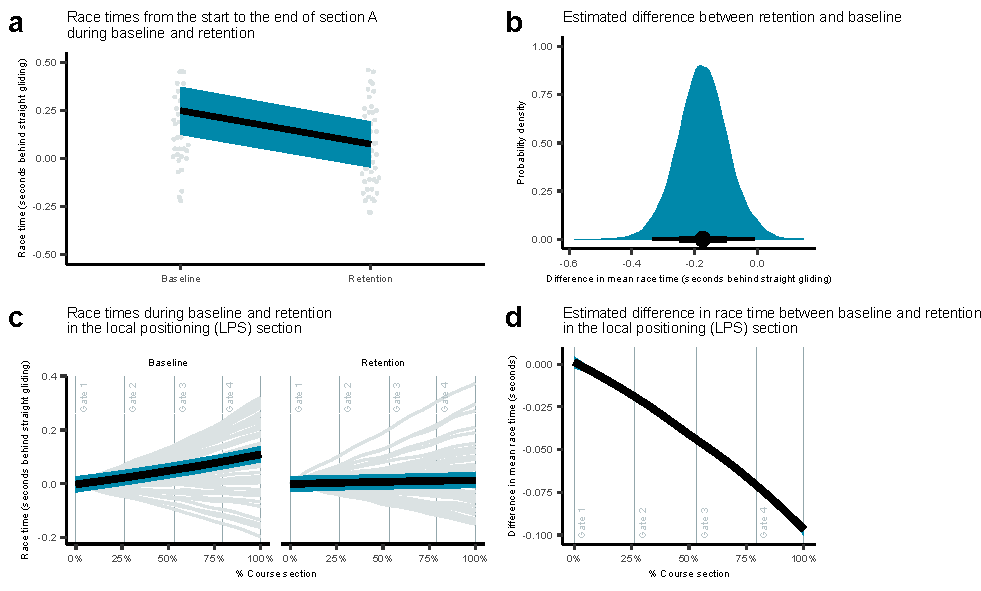
\includegraphics{figurer/figure_racetime_2.pdf}
\caption{Race times for both the intermediate time section and the local positioning system section. \textbf{a}. Estimated race times during baseline and retention for the intermediate time section. \textbf{b}. Estimated differences (contrast) between baseline and retention for the intermediate time section. \textbf{c}. Estimated race times during baseline and retention for the local positioning section. \textbf{d}. Estimated differences (contrast) between baseline and retention for the local positioning section. The black lines denote the expected mean or differences in mean, with the shaded area representing their 95\% credible interval (CI). Each gray point or line represents one run trial by a skier.}\label{fig: racetimes}
\end{figure}

\subsection{Velocity}
If the improvement in the skiers' race times can be attributed to the pumping mechanism, we would expect skiers to increase their velocity around or immediately after gate passage, at the time when the extension movement occurs.  Figure \ref{fig: velocity}a shows the velocity profiles for the local positioning system section during baseline and retention. We first describe the average velocity trend at baseline and then the contrast between baseline and retention.

Before the intervention (baseline), the skiers' velocity almost declined for every gate in the local positioning section compared to their velocity during straight gliding. With the exception of a slight velocity increase of 0.05 m/s (95\% CI [-0.08, 0.17]) from gate 1 to gate 2, the velocities decreased on average by -0.06 m/s (95\% CI [-0.19, 0.07]) from gate 2 to gate 3 and by -0.12 m/s (95\% CI [-0.25, 0]) from gate 3 to gate 4 compared to straight gliding times. We focused only on comparisons at the gates because the gates mark a fixed reference point. 

After the training intervention, skiers increased their entry velocity into the local positioning section (gate 1) by an average of 0.24 m/s (95\% CI [0.19, 0.29]) compared to the baseline velocity. However, the skiers also tended to increase their velocity throughout the section. Specifically, the skiers increased their velocity on average by 0.07 m/s (95\% CI [0.01, 0.12]) from gate 1 to gate 2, followed by a slight decrease of -0.02 m/s (95\% CI [-0.05, 0.02]) from gate 2 to gate 3. Subsequently, the velocity of the skiers increased again by 0.1 m/s (95\% CI [0.06, 0.14]) from gate 3 to gate 4. Therefore, the velocity of the skiers increased almost incrementally from gate to gate. Besides, the velocity profiles appeared wavier, as depicted in Fig. \ref{fig: velocity}b. In general, the pattern of these waveforms was that skiers increased their velocity after gate passage and continued to rise until the skier was between two gates. After that, the velocity decreased to gate 6 before it rose again. 

\begin{figure}
    \centering
    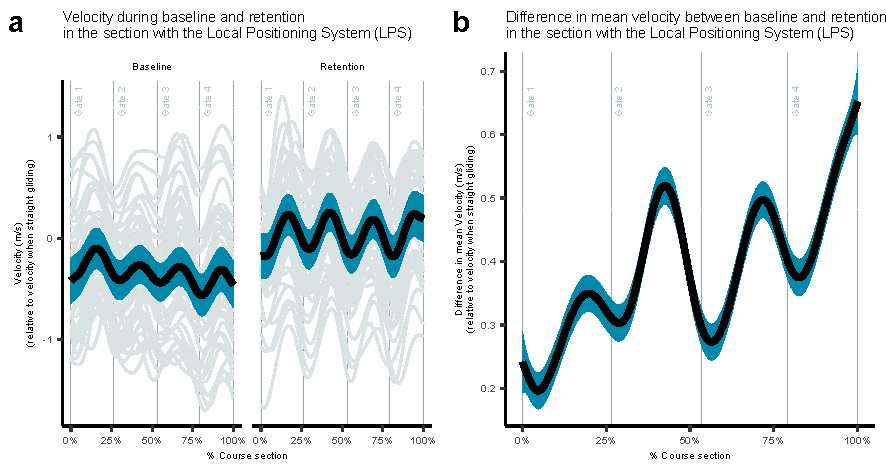
\includegraphics[width=1\linewidth]{figurer/figure_velocity_2.pdf}
    \caption{Velocity in the local positioning system section. \textbf{a.} Estimated velocity during baseline and retention for the local positioning section. \textbf{b}. Estimated differences (contrast) between baseline and retention for the local positioning section. The black lines denote the expected mean or differences in mean, with the shaded area representing their 95\% credible interval (CI). Each gray line represents one run trial by a skier}
    \label{fig: velocity}
\end{figure}

\subsection{Path length}
Finally, we analyzed the path length, which we expected not to undergo massive changes according to our measurements from the local positioning system. 

%In the case of change, we would expect it to be shorter during retention than during baseline because the skiers had learned to extend the center of mass toward the axis of rotation during the turn (theoretically).

At baseline, we found that the total path length from gate 1 to gate 2 was 91.53 (95\% CI [83.86, 99.30]), 92.57 (95\% CI [84.75, 100.45]) from gate 2 to gate 3, and 87.30 (95\% CI [79.40, 95.32]) from gate 3 to gate 4, while it was 69.30 (95\% CI [61.35, 77.16]) from gate 4 to the end of the section. Notably, the reason for the lower estimate from gate 4 to the end is that this section was shorter than the other sections. Fig. \ref{fig: path}a shows the total path length during each gate in the local positioning section.


\begin{figure}[H]
    \centering
    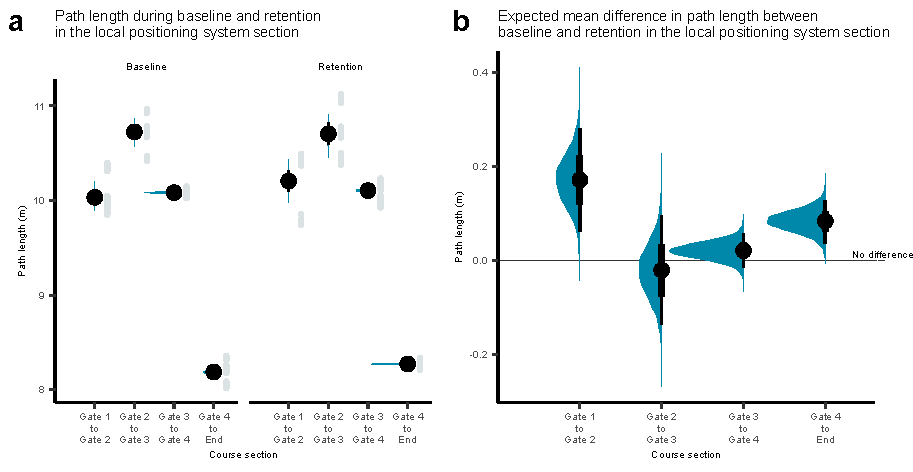
\includegraphics[width=1\linewidth]{figurer/figure_path2.pdf}
    \caption{Total gate-to-gate path length in the local positioning system section.\textbf{a.} Estimated gate-to-gate path length during baseline and retention for the local positioning section. \textbf{b}. Expected mean difference in gate-to-gate path length between baseline and retention in the local positioning section. The black lines denote the expected mean or differences in mean, with the shaded area representing their 95\% credible interval (CI). Each gray point represents one run trial by a skier}
    \label{fig: path}
\end{figure}

As expected, we found only marginal differences between baseline and retention in total path length. The expected mean difference was -2.73 (95\% CI [-13.8, 8.23]) from gate 1 to gate 2, -2.08 (95\% CI [-12.9, 8.99]) from gate 2 to gate 3, and -1.99 (95\% CI [-13.3, 9.18]) from gate 3 to gate 4, while it was -1.4 (95\% CI [-12.3, 9.62]) from gate 4 to the end of the section. Thus, there was considerable overlap in the expected differences in the mean difference in total path length. Fig. \ref{fig: path}b shows the expected mean difference in total path length during each gate in the local positioning section.

\section{Discussion}

Slalom racers rely on effective strategies to bring them down the course in the shortest amount of time possible. One strategy that skiers can employ to achieve this goal is to pump themselves to higher velocities by extending their center of mass closer to the axis of rotation during turns. However, researchers previously believed that these extension movements had little or negligible impact on skiers' race times. However, this view has been challenged by conflicting evidence in recent years. In a previous training intervention, we trained skiers on this pumping strategy and found that they greatly improved their race time in the course. This improvement could in principle be driven by two kinematic changes: either by skiing a shorter path length or by increasing the velocity. Here, we asked which of these best served as a plausible explanation of our data and examined the kinematic changes following the intervention. For this purpose, we employed a Bayesian estimation approach. We found that the training intervention likely exerted a greater impact on the skiers' velocity and acceleration through the turns than on the total path length.

To begin, the skiers' velocity turn profiles fluctuated during both the baseline and retention sessions, with their velocity increasing roughly at the gate passage, peaking around the switch to the next turn, before declining until the next turn. These wavy profiles closely align with previous observations of elite slalom racers skiing flat courses \cite{supej_impact_2015} and therefore seem to characterize skilled performers skiing slalom sections in flat terrain. In the retention test, we found notable shifts in the skiers' velocity profile. This expected shift was an increased velocity just after the gate passage. This velocity continued to increase until reaching its peak during the transition between two turns before declining just after the gate passage. Although we cannot provide quantitative data on the movements of skiers, the changes in velocity profile are consistent with the principles of pumping to increase velocity. According to these mechanics, when the skiers move their center of mass closer to the axis of rotation of the turn while the skis are edged and provide support, we would expect them to increase their rotational kinetic energy, which would positively affect their tangential velocity out of a turn \cite{lind_physics_2013}. This effect is likely observed in the velocity curves.

In contrast, we found little evidence that the total path length changed significantly from baseline to retention, as there was a large overlap in the expected mean difference between baseline and retention. A slight difference favored a shorter total path length at retention, but this difference was marginal. It is possible that this slight difference arises from a shorter path length when skiers extend their center of mass toward the axis of rotation in turn. We are unable to quantify this assumption with our data, but it warrants further investigation. Overall, our results are consistent with previous studies indicating that velocity through turns is a crucial performance factor \cite{federolf_quantifying_2012, supej_differential_2008, sporri_turn_2012, lesnik_best_2007}, and that the intervention's effect on pumping likely operated through this mechanism.

Our findings may have important practical implications for coaches. Based on this and prior studies \cite{christian_magelssen_reinforcement_2024}, pumping could be a crucial strategy for increasing velocity on flats in slalom. The great challenge for coaches lies in guiding skiers
to understand when pumping is an appropriate strategy and when it is not. 

\subsection{Limitation}
A limitation of the study is the low sampling frequency of the local positioning system, which is much lower than the minimum recommendation for studying the skiing technique in alpine skiing (10 Hz versus the 50 Hz, which is typically used in skiing  \cite{federolf_quantifying_2012}). Notably, the speed of the skiers in our study was in the lower range of a typical outdoor race course in slalom. Therefore, the system's accuracy may have been adequate for the conditions present in this study. Another limitation of the data is that the local positioning system only records data in two dimensions ($X$ and $Y$), which is sufficient for studying kinematics on flat terrain. However, alpine skiing involves a third dimension ($Z$), the slope of the terrain and vertical actions of the skiers. We addressed the former of these issues by measuring the altitude position of the gates and interpolating values between them. It is possible that this solution resulted in a loss of important data precision. Last, we encountered challenges in using the local positioning system in the ski hall due to the narrow space in the ski hall that made the nodes come too close to the walls. Due to this proximity, we lost over half of the turns and the upper part of the course. Only when the ski hall opened did we get data of sufficient quality for which we could analyze. Nevertheless, we observed several spikes in the signals, which we have openly and transparently reported. Despite these issues, the data from the study were deemed important to report.  We recommend that other researchers exercise caution and carefully consider whether and how to use local positioning systems in alpine skiing.

\section{Conclusion}
To conclude, we found that a training intervention aimed at pumping was more likely to impact the velocity and acceleration profiles of skiers and, to a lesser extent, their total distance traveled. Based on this and previous studies \cite{christian_magelssen_reinforcement_2024}, skiers can benefit greatly from pumping to achieve a higher velocity in situations where the available potential energy is low. However, there is a point where skiers have too much energy, and pumping becomes an inefficient strategy. Assisting skiers in linking the right strategy to the right situation is crucial for helping them develop sport expertise \cite{krakauer_motor_2019}.



%We chose to study the kinematic changes among the skiers in this section, as we observed time differences between baseline and retention. Om skikjørernes strekkbevegelse mot svingens axis of rotation fra lateralt innoverlent posisjon øker hastigheten vil vi forvente en økt hastighet rett etter svingen. Figure \ref{fig: velocity}a displays the velocity profiles for the LPS section at baseline and retention. During baseline, velocity declined relative to the velocity when straight gliding (From gate 1 to gate 4, the velocity decreased by -0.14 m/s (95\% CI [-0.36, 0.09]).


%The third strategy that can potentially make skiers faster on flat slopes in slalom is to 'extend,' also referred to as 'pumping' to increase velocity \cite{lind_physics_2013}. By moving closer to the axis of rotation of a turn from a laterally inclined position, the skier can boost its kinetic rotational energy under certain situations. According to Lind and Sanders \cite{lind_physics_2013} model, the skier achieves this effect by shortening the radius of the axis about which they rotate, which will reduce the moment of inertia and consequently increase the rotational kinetic energy of the system under the assumption that angular momentum is conserved. In their model, the gain in rotational kinetic energy from this motion is proportional to the amount of work the skier does against the centrifugal force; therefore, a larger extension movement will accomplish a greater increase in rotational kinetic energy.



%Vi forventet at skikjørernes forbedrede tider skyltes 



%A key explanation behind the improvement in skiers through the LPS-section was that they pumped themselves to higher velocities. Consistent with pumping contributing to a velocity increase after its execution, we predicted that a large velocity increase around the gate passage, caused by the intervention.

%Figure \ref{fig: velocity}a displays the velocity profiles for the LPS section at baseline and retention. During baseline, velocity declined relative to the velocity when straight gliding (From gate 1 to gate 4, the velocity decreased by -0.14 m/s (95\% CI [-0.36, 0.09]).

%After the intervention, we observed a large change in the velocity profile (Figure \ref{fig: velocity}b). We found that skiers had a higher entry velocity at retention. The expected average difference was 0.24 (95\% CI [0.19, 0.29]) at the first gate in the section. However, we also identified a global trend indicating that skiers continued to increase their velocity throughout the section. The expected difference in increase from gate 1 to gate 4 was 0.16 m/s (95\% CI [0.10, 0.21]).

%Den tydeligste endringen var likevel rett etter porten. Etter intervensjonen var hastighetsprofilen betydelig mer bølgeformet med store. Den forventede økningen mellom


\appendix

\section{Course setting}\label{appendixa}
This appendix describes how we set up the slalom courses for data collection. We began by laying out a 50-meter long rectangular square. This was consistently extended from a fixed reference point at the top of the course, ensuring that the starting position remained constant. The placement of the square along the course was performed through visual aiming with a fixed reference point on the ceiling. Once we had found the right position and angle, we placed the rectangular square down on the snow surface. For every 10 meters of the rope, we had a tape mark on both ends of the rope to indicate the vertical distance of the course. Then, we lay a second rope between these two tape points with tape points where to set the different courses (that is, their offset). Fig. \ref{fig: coursesetting} shows an illustration of how this process worked.




\begin{figure}[H]
\centering
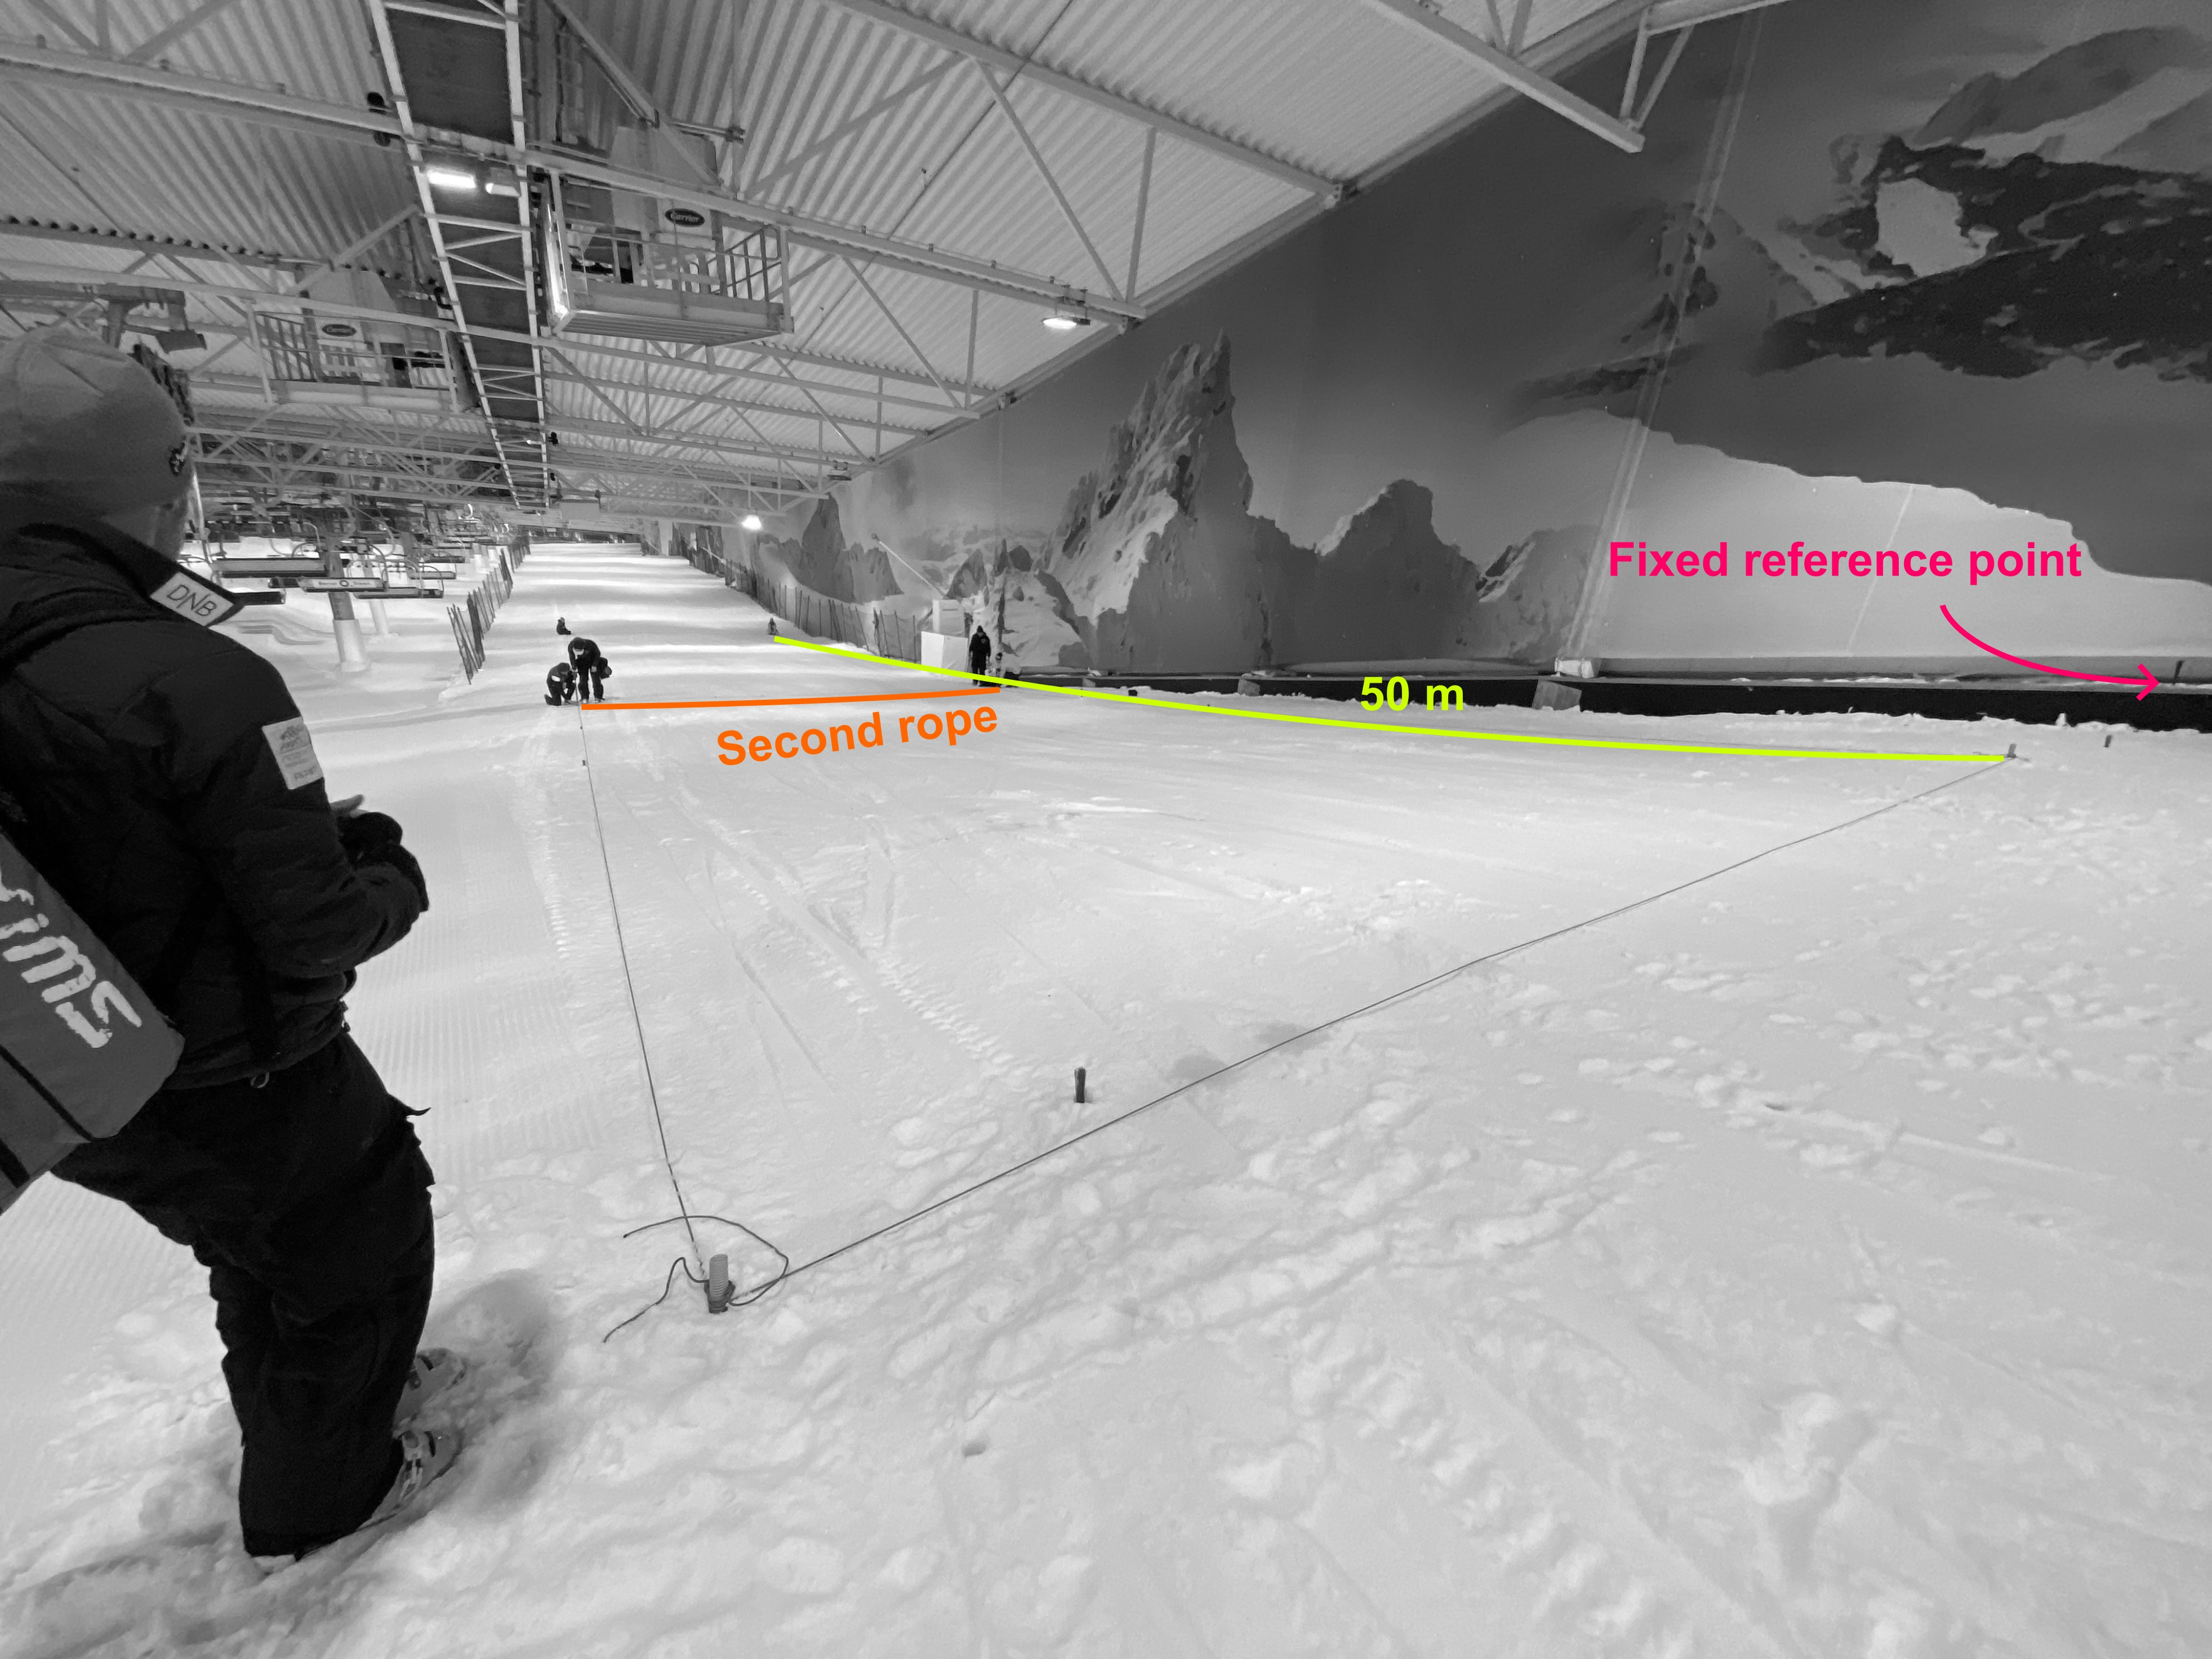
\includegraphics{figurer/figure_appendix_course.jpg}
\caption{Illustration of the course setting. This is an image from one of the training session with the staff}\label{fig: coursesetting}
\end{figure}



\section{Courses and local positioning system} \label{appendixb}
Skal vi skrive noe her?


\begin{figure}[H]
\centering
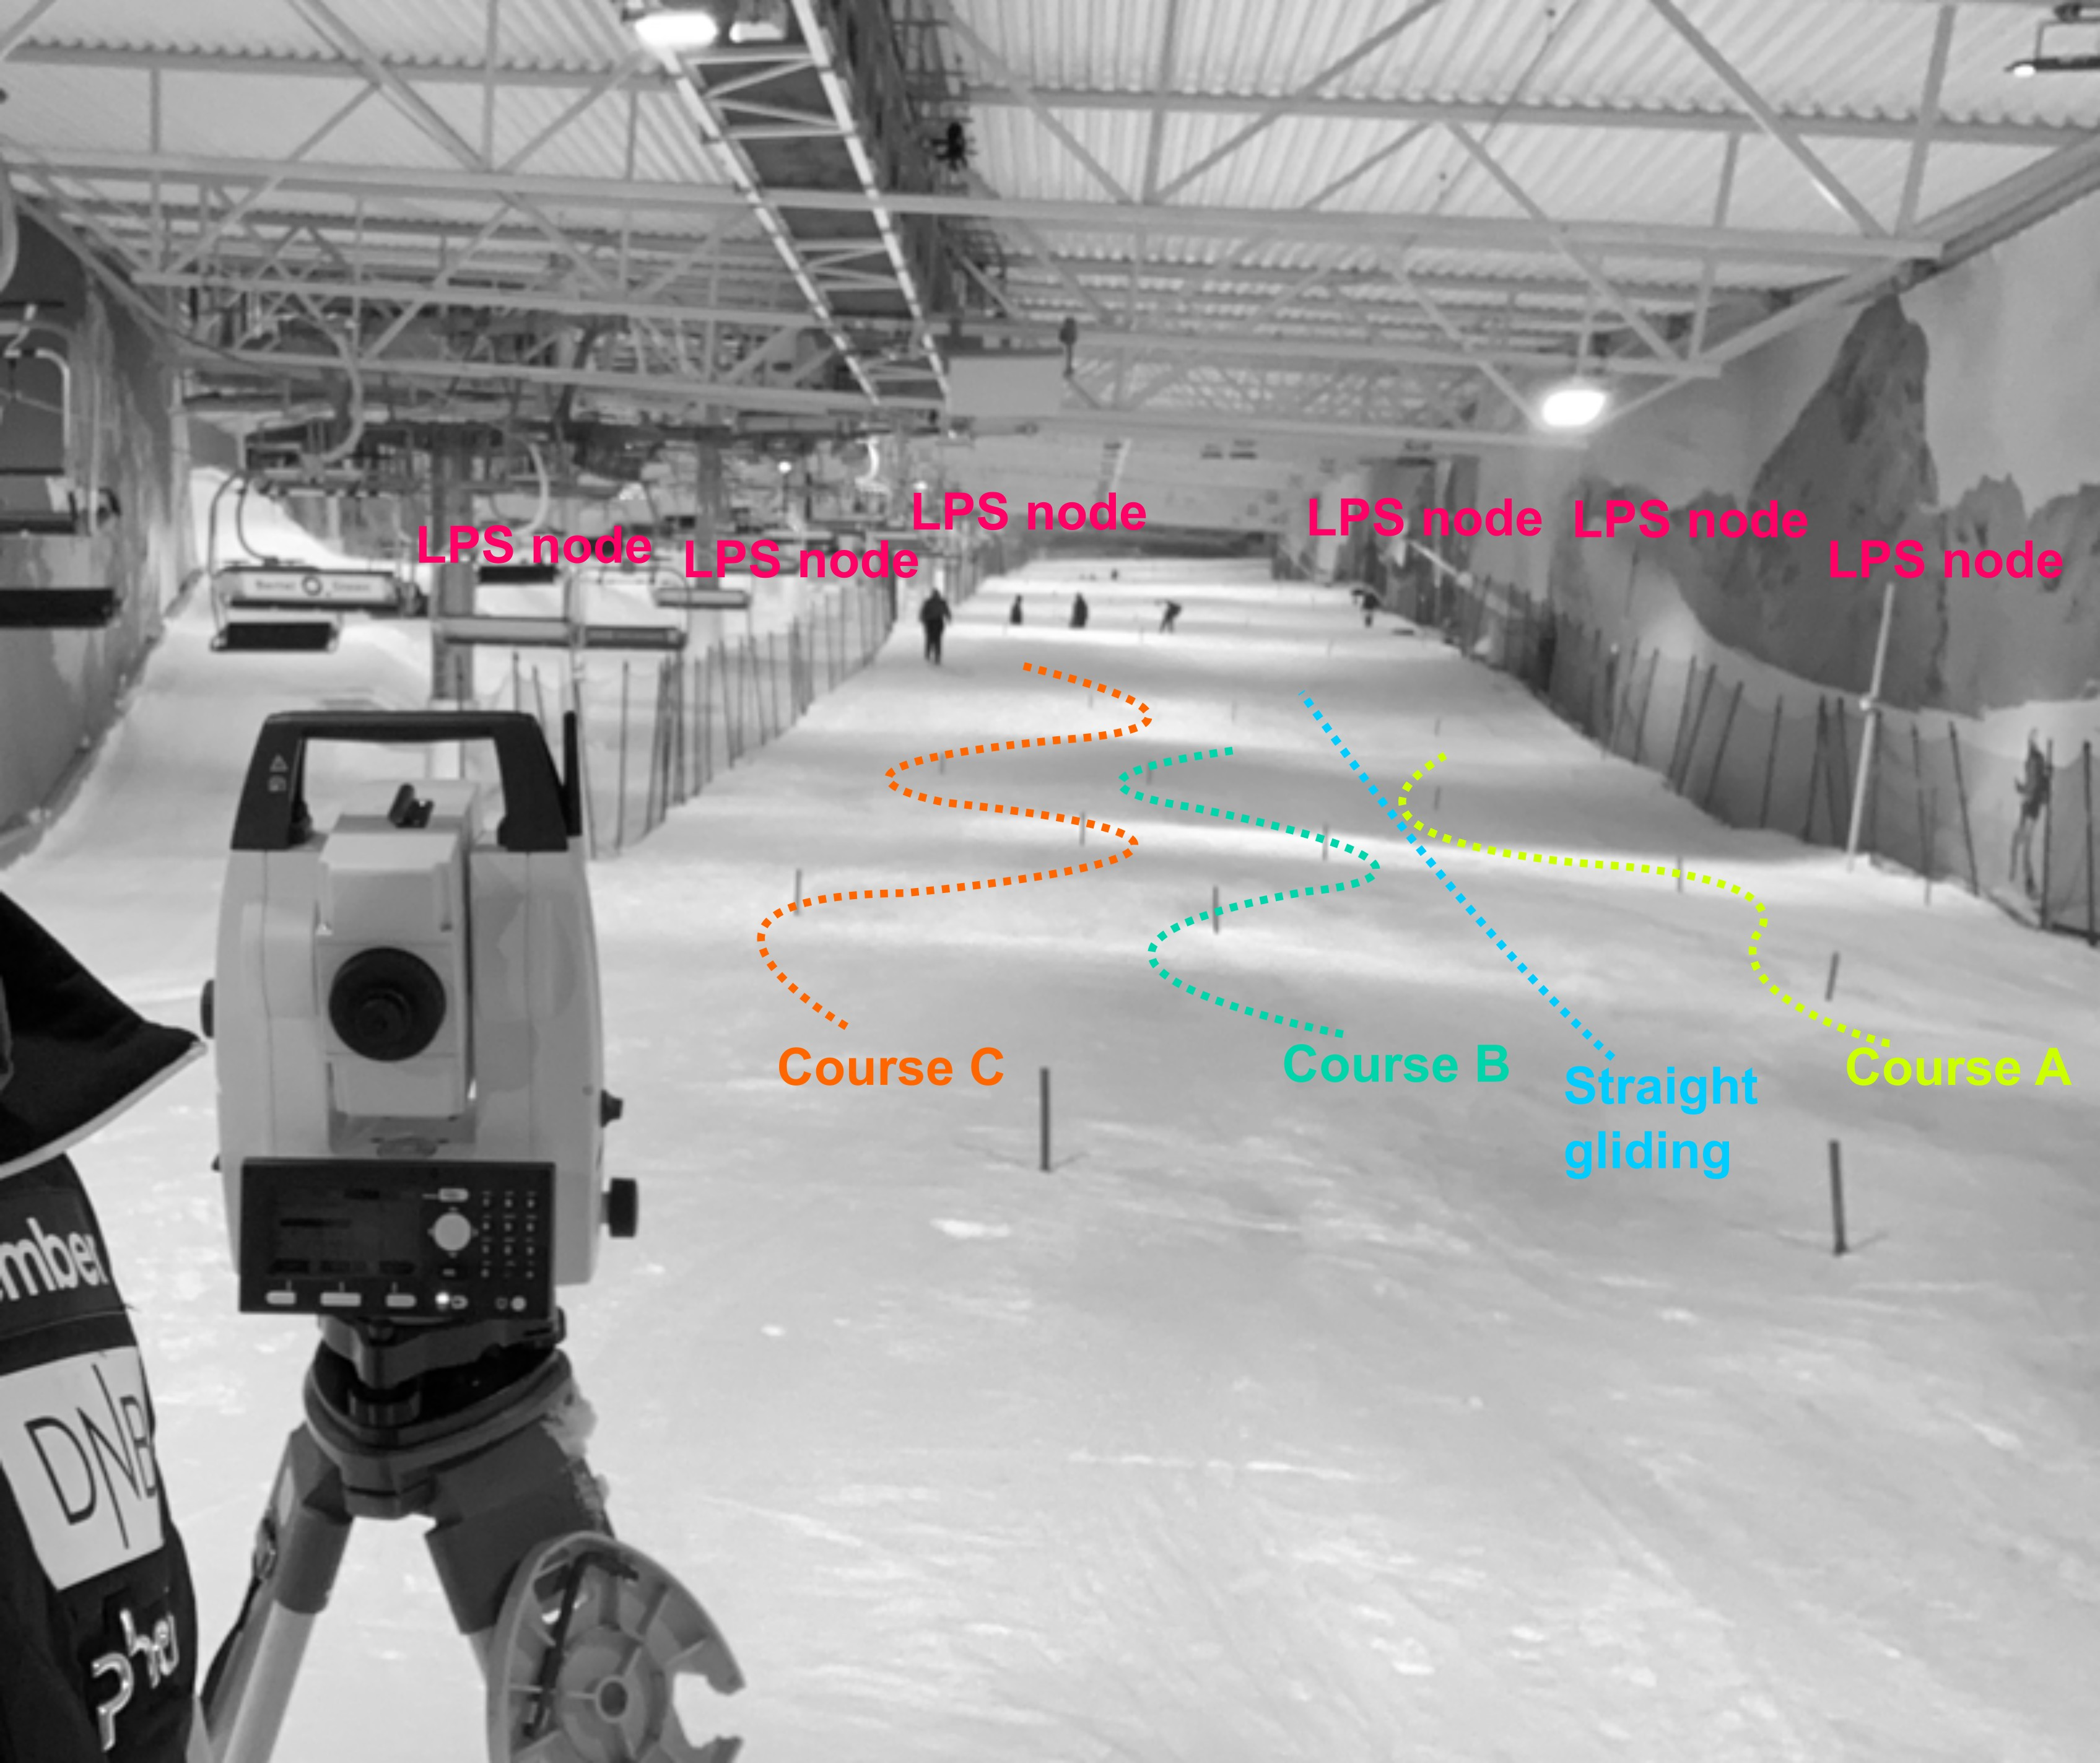
\includegraphics{figurer/figure_appendix_LPS.jpg}
\caption{Illustration of the course and the local positioning system setup}\label{fig: coursesetting}
\end{figure}




\section{Details of statistical models}\label{appendixc}

Model 1: Race times during baseline and retention in the intermediate section

\begin{verbatim}
brm(
family = gaussian,
formula = racetime ~ 0 + session + 
          (0 + session | skier),
prior = c(prior(normal(0, 1), class = b),
          prior(exponential(1), class = sigma),
          prior(exponential(1), class = sd)),
control = list(adapt_delta = 0.95))
\end{verbatim}


Model 2: Race times during baseline and retention in the local positioning section

\begin{verbatim}
brm(family = gaussian,
    formula = bf(racetime ~ 1 + session + 
                 s(sectionlength, by=session) +
                 s(sectionlength, skier, bs="fs", m=1)),
    prior = c(prior(student_t(10, 0, 1), class=Intercept),
              prior(student_t(10, 0, 1), class = b),
              prior(student_t(10, 0, 1), class = sds),
              prior(exponential(1), class = sigma)),
    control = list(adapt_delta = 0.95))
\end{verbatim}

Model 3: Velocity during baseline and retention in the local positioning section

\begin{verbatim}
brm(family = gaussian(),
    bf(velocity ~ 1 + session + 
       s(sectionlength, by=session, k=40) +
       s(sectionlength, skier, bs="fs",m=1, k=10)), 
       prior = c(prior(student_t(10, 0, 1.5), class = Intercept),
                 prior(student_t(10, 0, 1.5), class = b),
                 prior(student_t(10, 0, 1), class = sds),
                 prior(exponential(1), class = sigma)),
    control = list(adapt_delta = 0.95))
\end{verbatim}

Model 4: Acceleration during baseline and retention in the local positioning section

\begin{verbatim}
brm(family = gaussian(),
    bf(acceleration ~ session + 
       s(sectionlength, by=session, k=45) +
       s(sectionlength, skier, bs="fs",m=1, k=10)), 
    prior = c(prior(student_t(10, 0, 1.5), class = Intercept),
              prior(student_t(10, 0, 2), class = b),
              prior(student_t(10, 0, 1.5), class = sds),
              prior(exponential(1), class = sigma)),
    control = list(adapt_delta = 0.8))
\end{verbatim}

Model 5: Total acceleration during baseline and retention in the local positioning section

\begin{verbatim}
brm(family = gaussian(),
    formula = totalacceleration ~ 0 + acc_gate:session +
              (0 + acc_gate:session | skier),
    prior = c(prior(normal(0, 100), class = b),
              prior(exponential(1), class = sigma), 
              prior(exponential(1), class = sd)),
    control = list(adapt_delta = 0.95))
\end{verbatim}

Model 6: Total path length during baseline and retention in the local positioning section

\begin{verbatim}
brm(family = gaussian(),
    formula = pathlength ~ 0 + gate:session + 
            (0 + gate:session | skier),
    prior = c(prior(normal(100, 50), class = b), 
              prior(exponential(1), class = sigma),
              prior(exponential(1), class = sd)),
    control = list(adapt_delta = 0.95))
\end{verbatim}

\section{Challenges with the local positioning system} \label{appendixd}
We encountered challenges with local positioning system in the ski hall, especially in the upper part of the course. Only when the hall opened up, increasing the distance between the node and the wall, did we receive a signal strong enough to provide us with analyzable data. However, we still faced some signal issues. We have thoroughly analyzed and plotted all the data, and this overview is available as both a quarto and html file at OSF  


\begin{figure}[H]
\centering
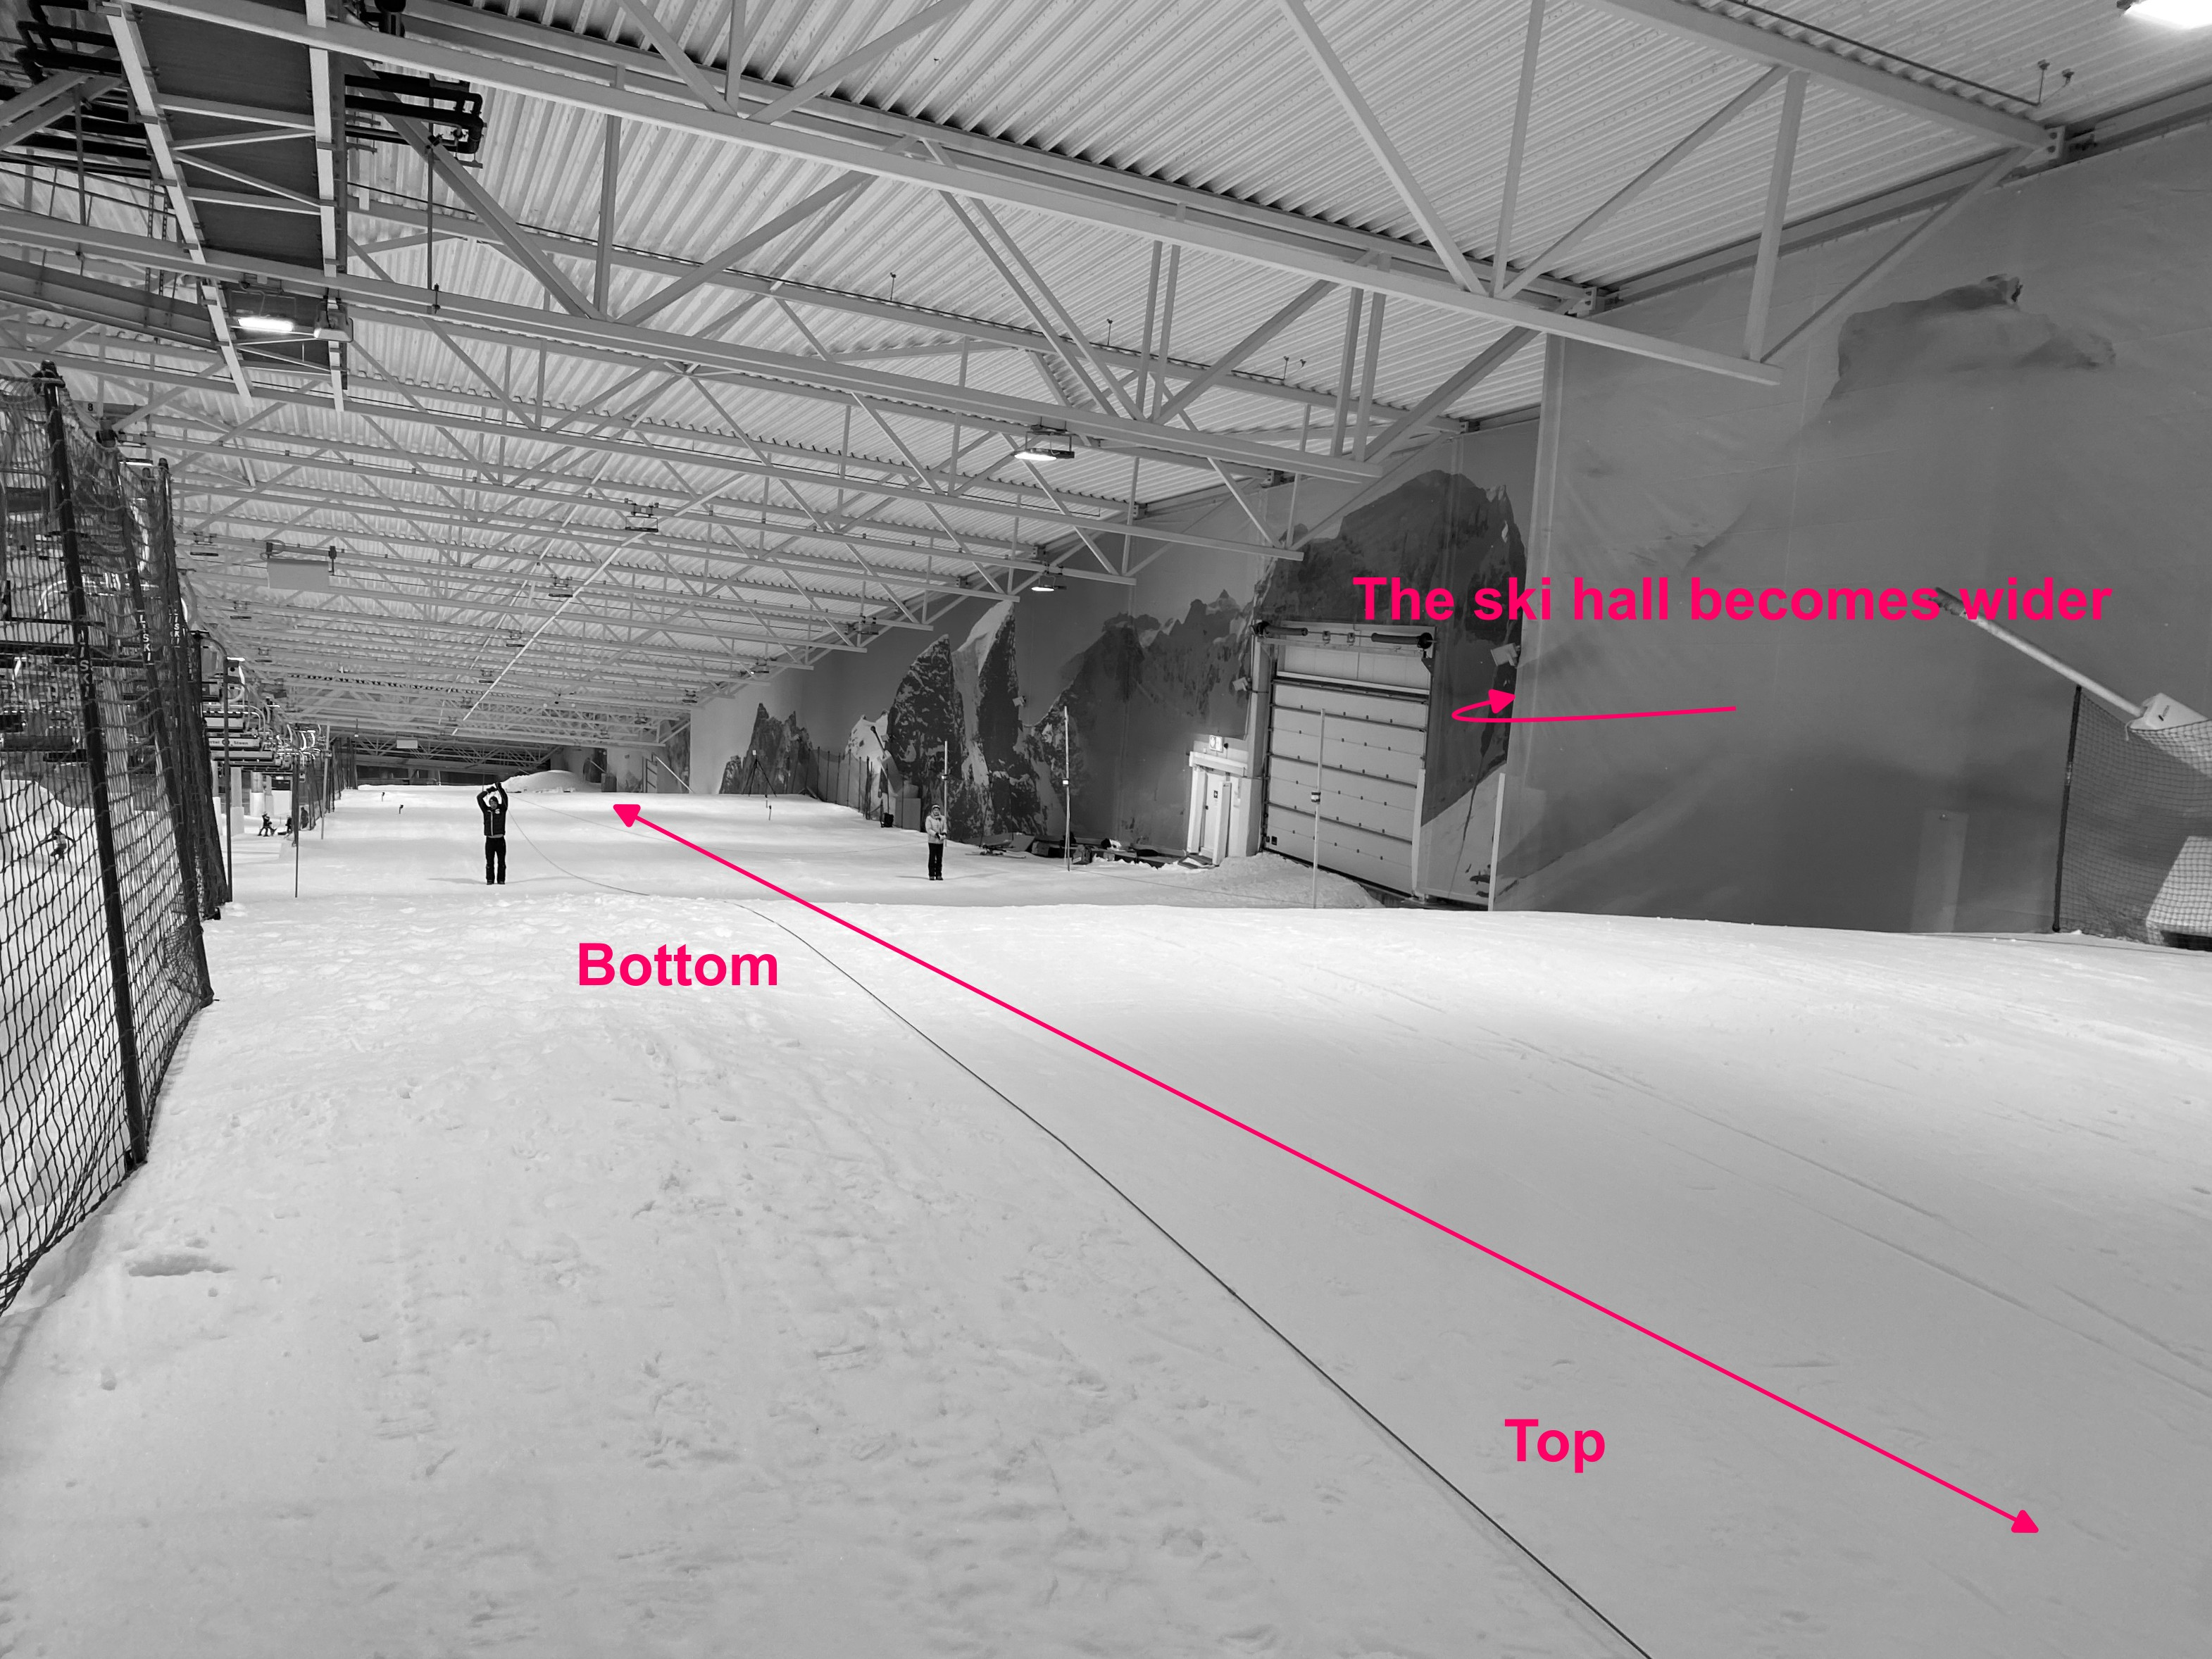
\includegraphics{figurer/figure_appendix_LPS_wide.jpg}
\caption{Illustration of the lower part in the local positioning section.The picture was taken in conjunction with course setting}\label{fig: lpsissues}
\end{figure}



\section{Acceleration data}

\subsection{Acceleration}
We continued examining acceleration through the turn to analyze the velocity changes more closely. As shown in Fig. \ref{fig: acc}a, the acceleration exhibited fluctuating waves, with skiers increasing their acceleration up to about the switch between two turns that began just before or around the gate passage. After this switch, the skiers decelerated until just before the gate. 

During the baseline, we found that the skiers' acceleration decreased on average by -0.91 m/s$^2$ (95\% CI [-1.71, -0.05]) from gate 1 to gate 2, followed by an increase of 0.42 m/s$^2$ (95\% CI [-0.40, 1.31]) from gate 2 to gate 3 and then a marginal increase of 0.01 m/s$^2$ (95\% CI [-0.84, 0.79]) again from gate 3 to gate 4, compared to the acceleration during straight gliding.

Following the intervention, the skiers developed a significantly more wavy acceleration profile with higher peaks and lower troughs compared to the baseline. We performed a gate-to-gate analysis, which revealed that acceleration was lower at gate 1 by -0.53  m/s$^2$ (95\% CI [-0.66, -0.41]), at gate 2 by -0.19  m/s$^2$ (95\% CI [-0.26, -0.13]), at gate 3 by -0.48  m/s$^2$ (95\% CI [-0.54, -0.42]), and at gate 4 by -0.42  m/s$^2$  (95\% CI [-0.48, -0.36]) compared to the baseline. Fig. \ref{fig: acc}b shows the expected mean difference between baseline and retention. 

To better understand how the acceleration changed between baseline and retention in each turn, we computed the total acceleration from gate to gate through the local positioning sequence. From this model, we found that the estimated difference in total acceleration was 24.4 (95\% CI [-14.4, 63.1]) from slalom gate 1 to slalom gate 2, 1.65 (95\% CI [-37.6, 40.1]) between gate 2 and gate 2, 39.4 (95\% CI [0.59, 78.1]) from gate 3 to gate 4, and 107.0 (95\% CI [68.8, 146.0]) from gate 4 to the end of the sequence. Therefore, the skiers appears to have had a positive overall acceleration in most of the gates in the sequence. Fig. \ref{fig: acc}c and d show the total acceleration during each gate in the local positioning section.

\begin{figure}[H]
\centering
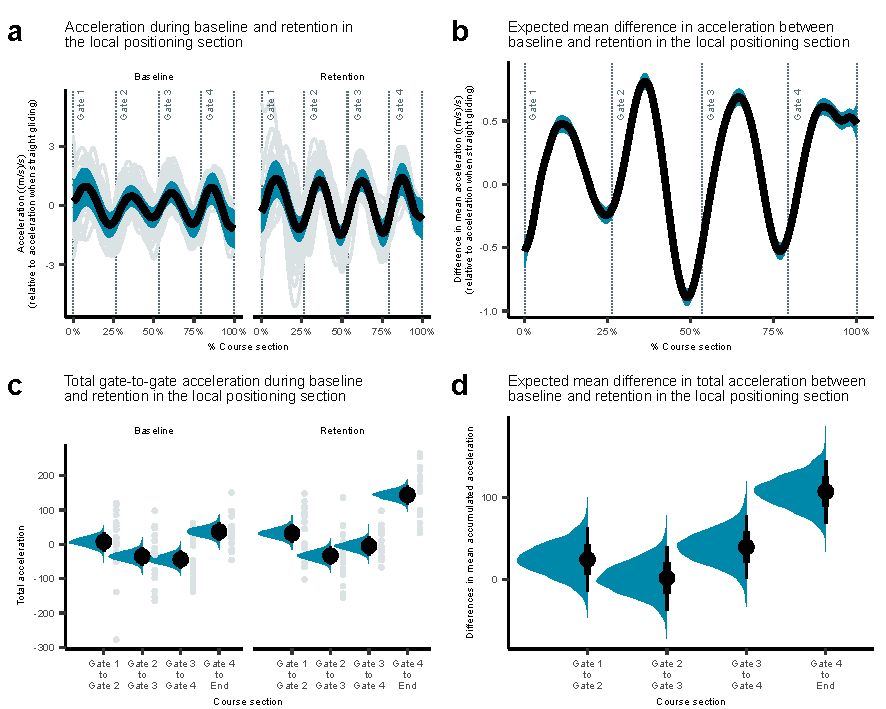
\includegraphics{figurer/figure_acc_2.pdf}
\caption{Acceleration in the local positioning system section.\textbf{a.} Estimated acceleration during baseline and retention for the local positioning section. \textbf{b}. Expected mean difference between baseline and retention in the local positioning section.\textbf{c.} Estimated total gate-to-gate acceleration during baseline and retention in the local positioning section. \textbf{d}. Expected mean difference between baseline and retention in the local positioning section. The black lines denote the expected mean or differences in mean, with the shaded area representing their 95\% credible interval (CI). Each gray point or line represents one run trial by a skier}\label{fig: acc}
\end{figure}




\printbibliography %Prints bibliography

\end{document}
